\documentclass[a4paper,12pt]{article}
\usepackage{epsfig,amssymb,amsmath,}
\usepackage{color}

\textwidth=18cm%6.25true in
\textheight=24.5cm%9.65true in
\voffset=-2.5cm%-1true in
\hoffset=-0.75true in

%%%%%%%%%%%%%%%%%%%%%%%%%%%%%%%%%%%%%%%%%%%%%%%%%%%%%%%%%%%%%%%%%%
%\usepackage[sorting=none, url=false, style=numeric-comp]{biblatex}
%\bibliography{../global.bib}
%%%%%%%%%%%%%%%%%%%%%%%%%%%%%%%%%%%%%%%%%%%%%%%%%%%%%%%%%%%%%%%%%%
\usepackage[sort&compress,numbers]{natbib}
\bibliographystyle{apsrev4-1}
\usepackage{doi}%<----------
% https://tex.stackexchange.com/questions/15677
%%%%%%%%%%%%%%%%%%%%%%%%%%%%%%%%%%%%%%%%%%%%%%%%%%%%%%%%%%%%%%%%%%

\usepackage{tikz}
\usetikzlibrary{arrows}
\usepackage[]{hyperref}     
%\hypersetup{citecolor = blue, linktocpage=true}
\usepackage{titlesec}
\titleformat{\subsection}
{\normalfont\large\bfseries}{\thesubsection}{1em}{}

\usepackage{graphicx} % Allows including images    
\graphicspath{{../figures/}, {../figures/growthrates/}}

\renewcommand{\bf}{\mathbf}
\renewcommand{\cal}{\mathcal}
\newcommand{\pd}[2]{\frac{\partial #1}{\partial #2}}
\newcommand{\pdn}[3]{\frac{\partial^{#3} #1}{\partial #2^{#3}}}
\newcommand{\pdop}[1]{\frac{\partial}{\partial #1}}
\newcommand{\nd}[2]{\frac{d #1}{d #2}}
\newcommand{\ndn}[3]{\frac{d^{#3} #1}{d #2^{#3}}}
\newcommand{\ndop}[1]{\frac{d}{d #1}}
\newcommand{\dt}{\frac{d}{dt}}
\newcommand{\half}{\frac{1}{2}}
\newcommand{\third}{\frac{1}{3}}
\renewcommand{\th}[1]{\frac{1}{#1}}
\newcommand{\ex}[1]{\left\langle #1 \right\rangle}
\renewcommand{\d}{\delta}
\renewcommand{\l}{\ell}
\renewcommand{\t}{\tau}
\newcommand{\ket}[1]{\left|#1\right\rangle}
\newcommand{\bra}[1]{\left\langle#1\right|}
\newcommand{\braket}[2]{\left\langle#1\middle|#2\right\rangle}
\newcommand{\brakett}[3]{\left\langle#1\middle|#2\middle|#3\right\rangle}
\newcommand{\nn}{\nonumber\\}
\newcommand{\note}[1]{{\color{red}{#1}}}

\DeclareMathOperator{\Tr}{Tr}
\let\Re\relax
\DeclareMathOperator{\Re}{Re}

\title{Thermalization and localization in random unitary circuits}
\author{Charles Stahl}

\begin{document}

\maketitle

\section{Introduction} \label{sec:intro}

In this essay we will discuss the quantum dynamics of closed systems, showing that the two late-time possibilities are thermalization and localization. We will then describe how to study these processes using random unitary circuits. Sec.~\ref{sec:ruc} presents various methods of describing dynamics in thermalizing circuits. The majority of circuits currently described in the literature thermalize, although this is not a necessity. One path to localization in random unitary circuits is through fractonic conservation laws. To motivate these we will introduce fractonic systems in Sec.~\ref{sec:frac} and show how they naturally conserve higher moments of charges. Finally, in Sec.~\ref{sec:fraccirc} we will show that circuits that conserve these higher moments of charge indeed localize. We will follow the results of~\cite{PaiFracton}, and in fact the first 4 sections of this essay are designed to build to these results. Sec~\ref{sec:conc} reviews the broad structure of this essay and presents some possibilities for future research.

\note{Include term ``scrambling"}


\section{Quantum dynamics of closed systems} \label{sec:dyn}

This section will serve to introduce the reader to the basics of quantum dynamics of closed systems. It will closely follow Ref.~\cite{Nandkishore14}, drawing on other sources for examples.

I'll cover operator spreading here, although some of that material may belong in the RUC section. Other sources include~\cite{GogolinStatMech, PolkovnikovClosed, Cazalilla2010}.

\subsection{Closed quantum systems} \label{sub:closed}

Quantum statistical mechanics usually considers a quantum system coupled to a bath. As in classical statistical mechanics, this allows the system to exchange energy and conserved charges with the bath. Additionally, the system may become entangled with the bath, leading to dephasing. Then, as in the classical case, the state of the system at long time (is|may be approximated by) the thermal state, $\rho^{\text{th}}(T)=Z^{-1}(T)e^{-H/T}$. 

Sometimes these systems are integrable\dots

\subsection{Thermalization and localization} \label{sub:therm}

Since the bath itself is quantum mechanical, we could consider the system and bath together as a single closed quantum system. We will take this perspective for the remainder of the essay, referring to the original system as some subsystem. The study of closed quantum systems has expanded recently, driven by experimental, numerical, and theoretical motivations~\cite{GogolinStatMech}.

I'll discuss the ETH here as it seems to be an important enough result, but I don't think it's strictly necessary for the flow of the essay.

I'll continue to follow the Nandkishore review for this section and the section on MBL.

\subsection{Operator spreading as a measure of dynamics} \label{sub:opsp}

How can we measure dynamics?
Can we look at how states evolve?
This is tempting, but we would need a background\dots

We will look at how initially local operators spread in time. They will evolve in the Heisenberg picture\dots

Two measures of the spreading of an operator are the right weight density $\rho_R(i,t)$ and the OTOC $C(i,t)$.

\subsection{Other measure of dynamics} \label{sub:other}

Other useful quantity is the bipartite entanglement entropy $S(i,t)$.
Other possible entropies: Renyi entropies.
Dynamics studied in~\cite{RakovskyDiff, HuangRenyi}.
Also mention~\cite{JonayEntanglement}.

I like the transition between thermalizing and localizing phases, so I'll spend some time on that, with sources~\cite{PalHuse, KhemaniCP}. Specifically, the fact that this is not a phase transition of the ground state, like we are used to, and different order parameters for the transition. 

\subsection{Many-body localization} \label{sub:mbl}

If there's time and space\dots


\section{Random unitary circuits and Floquet systems} \label{sec:circuits}

In this essay we will be considering the dynamics of Hamiltonian systems, quantum circuits, and Floquet systems. We have already assumed the reader is familiar with the evolution of operators under Hamiltonian dynamics, but here we will introduce quantum circuits and Floquet systems. Both have unitary evolution, but are in some sense less structured than Hamiltonians.

\note{Define ``physical" systems, disorder realization.}

\note{Haar measure}

\subsection{Random unitary circuits} \label{sub:ruc}

Quantum circuits, unsurprisingly, are the quantum analogue of classical circuits. As unitarity is a constraint on quantum evolution, they are also called unitary circuits. We will be interested in 

\subsection{Floquet systems} \label{sub:floq}

Theres a thorny issue that we brushed asie when we discussed systems without conserved quantities. We defined the systems by their Hamiltonians, but any system with a Hamiltonian conserves energy. As discussed in Sec.~\ref{sec:intro}, random circuits need not have any conserved quantities at all. How then can we compare them to any sort of Hamiltonian system?

The resolution lies in Floquet systems. In this branch of systems, there is a succession of Hamiltonians applied, each for a set amount of time. For example, if we ``turn on" Hamiltonian $H_1$ for time $T/2$ and then $H_2$ for $T/2$, then the Floquet unitary time evolution operator for one whole period of time $T$ is 
\begin{align}
U_F(T) = U_2\left(\frac{T}{2}\right)\; U_1\left(\frac{T}{2}\right) = e^{-i\frac{T}{2}H_2} e^{-i\frac{T}{2}H_1}.
\end{align}
For $t=nT$ with $n\in \mathbb{Z}$, the time evolution operator is $U(t)=U^n(T),$ while for noninteger multiples of $T$ it is more complicated. 

One example is the kicked Ising model~\cite{vonKeyserlingkHydro}, with 
\begin{align}
H_1 &= \phantom{h}\sum_i\left(Z_iZ_{i+1}+gZ_i\right),\nn
H_2 &= h\sum_iX_i. \label{eqn:kicked}
\end{align}
Note that all terms acting at a given time commute with each other. Therefore this Floquet model can be written as a unitary circuit (not random) with 2-site gates. 

Another example, from Refs.~\cite{ZhangFloq, ChenOtoc}, has time evolution operator 
\begin{align}
U_F(T) = e^{-i\frac{T}{2}H_x}e^{-i\frac{T}{2}H_z},
\end{align}
with
\begin{align}
H_x &= \sum_i g\Gamma X_j,\nn
H_z &= \sum_i \left[Z_iZ_{i+1} + (h+g\sqrt{1-\Gamma^2}G_i)Z_i\right],
\end{align}
where $G_i$ are independent Gaussian random variables. We will use the parameters $(g,h,T) = (0.9045,0.8090,0.8)$ throughout.
Note that as $\Gamma\to1$ this approaches the kicked Ising model, which thermalizes. As $\Gamma\to1$, this model becomes equivalent to the time-independent Hamiltonian $H=\sum_i\left[Z_iZ_{i+1} + h_iZ_i\right]$ with random field $h_i$, which is localized. For lack of a better term we will call this the $\Gamma$ model.

As in the previous section, we can study the transition between the localized and thermalizing phases by varying a parameter of the model, in this case $\Gamma$. Fig.~\ref{fig:floqtrans} demonstrates the transition using two diagnostics. 
\begin{figure}
	\centering
	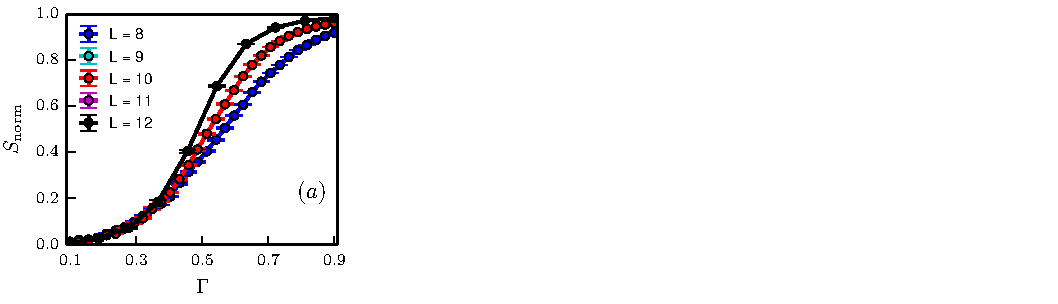
\includegraphics[width=.3\linewidth]{ZhangTransition1}
	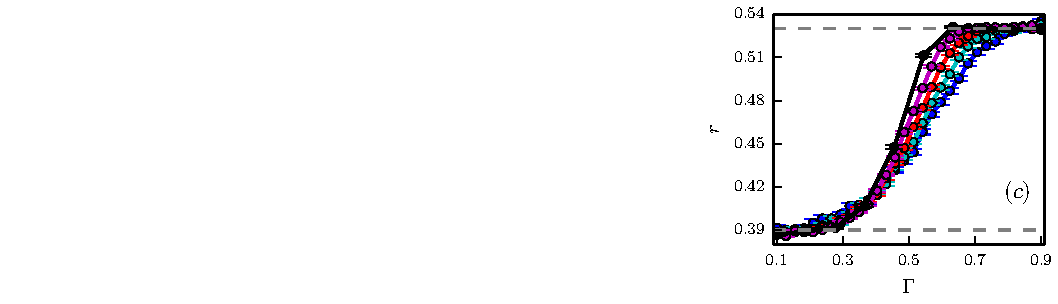
\includegraphics[width=.3\linewidth]{ZhangTransition2}
	\caption{Dynamical phase transition of the $\Gamma$ model. (a) demonstrates the phase transition through the average entanglement entropy between halves of the chain. (c) shows the same transition, but using the level statistics parameter. Figure from~\cite{ZhangFloq}.}
	\label{fig:floqtrans}
\end{figure}
The first is the entanglement entropy between two halves of the chain in energy eigenstates, 
\begin{align}
S_E \equiv -\Tr\{\rho_L\log\rho_L\} = -\Tr\{\rho_R\log\rho_R\},\label{eqn:Shalf}
\end{align}
where $\rho_L$ and $\rho_R$ are reduced density matrices of the right and left halves of the chain, with no relation to the operator right- and left-weights. The second equality in~\ref{eqn:Shalf} is due to the whole chain being in a pure state. The maximal possible entanglement between these halves is $S_\text{max}=L/2$, but random pure states will be close to the Page value~\cite{Page, ZhangTherm}
\begin{align}
S_R = \frac{L}{2} - \th{2\ln 2} -\mathcal{O}\left(\th{2^L}\right).
\end{align}

In the thermalizing phase the eigenstates have ``volume law" entanglement, close to $S_R$, while in the localized phase they have ``boundary law" entanglement, constant in $L$~\cite{ZhangFloq}. Therefore for large enough $L$, $S_E/S_R$ should distinguish between the phases. After averaging over all eigenstates for a given disorder realization and then averaging over disorder realizations, we arrive at $S_\text{norm} = \ex{S_E}/S_R$.

Alternatively we can use the level statistics parameter $r$ discussed previously. In the thermalizing phase the energies should be distributed according to the circular orthogonal ensemble with $r \approx 0.53$, while in the localizing phase the energies follow Poisson level statistics with $r\approx 0.39$. The dashed lines in Fig.~\ref{fig:floqtrans} show these values.

In Fig.~\ref{fig:floqtrans}, notice the agreement between the two diagnostics in the critical value $\Gamma_c$. Furthermore, both transitions become sharper for increasing $L$, as one would expect. The suggestion is that the transition is singular in the thermodynamic limit. In Sec.~\ref{sub:fncons} we will study this model at $\Gamma=.85$, deep in the thermalizing phase.


\section{Thermalization in systems with no conservation laws} \label{sec:ncons}

In this section I'll bring back the concepts of thermalization and show how they can be quantified in random circuits. For the actual construction of circuits I'll use~\cite{NahumRuhmanHuse, NahumEntanglement}.
For operator hydrodynamics I'll cite~\cite{NahumOpSp, vonKeyserlingkHydro, KhemaniLambda, KhemaniOpSp, JonayEntanglement}. Some of this material is not in RUCs though, so I still have to sort that out.

\subsection{Physical systems with no conservation laws} \label{sub:fncons}

As shown previously, the $\Gamma$ model with $\Gamma=0.85$ is deep within the thermalizing phase. Ref.~\cite{ChenOtoc} studied the OTOC of an initially local operator in this model. It uses a \note{slightly different definition of the OTOC...}

The key point is the exponential dependence of the OTO correlator. 
\begin{figure}
	\centering
	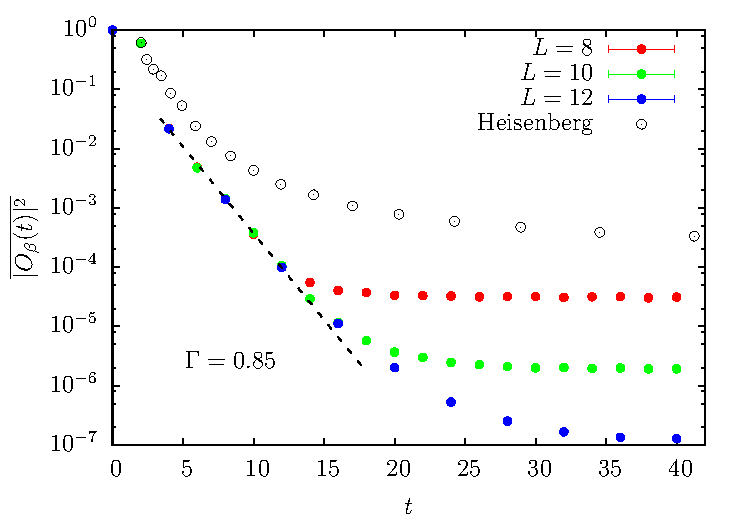
\includegraphics[width=.5\textwidth]{ChenExp}
	\caption{Exponential decay of the OTO correlator in a thermalizing Floquet model with no conserved charges~\cite{ChenOtoc}. For increasing system size, the decay continues to be exponential for a longer time before saturating. The black circles show the non-expenential decay of a Hamiltonian system. This decay is power-law, and will be discussed in the following section.}
	\label{fig:ChenExp}
\end{figure}
Fig.~\ref{fig:ChenExp} shows the exponential decay of the OTO correlator for various system sizes. Finite size effects cause the OTO correlator to saturate and therefore deviate from exponential behavior. However, the figure shows that this happens later for larger $L$, suggesting that the exponential decay continues for an arbitrarily long time for large enough $L$.

Ref.~\cite{vonKeyserlingkHydro} cranks $\Gamma$ all the way to 1, to study the kicked Ising model, defined in Eq.~\ref{eqn:kicked}. It goes beyond the early-time exponential dependence to study the saturation. The quantity under inspection is now the OTOC rather than the OTO correlator, so it should start at 0 and saturate to 1. There is also a focus on the operator right- and left-weights, $\rho_L$ and $\rho_R$.

Fig.~\ref{fig:vonKSpreading} shows the relevant quantities. Although it is for the quantum circuit, the qualitative behavior is the same (that's the whole point of this essay). At each site, exponential growth of both $\rho_R$ and the OTOC begins when the site enters the light cone. Exponential growth continues until the front reaches the site, at which point $\rho_R$ peaks and the OTOC begins to saturate. This front is the focus of Ref.~\cite{vonKeyserlingkHydro}.
Figs.~\ref{fig:vonKSpreading}~(a) and (b) can be thought of as horizontal slices though Fig.~\ref{fig:vonKSpreading}~(c). To compare with Fig.~\ref{fig:ChenExp}, imagine a vertical slice through~\ref{fig:vonKSpreading}~(c), with $t=0$ occurring at the position of the light cone.

The results, found through numerical simulation, are that the front propogates linearly at a velocity called the butterfly velocity, $v_B$. Consider $\rho(i,t)$. For $t<<v_B i$, the spreading operator has not yet reached $i$ and $\rho(i,t)$ is small. As the peak passes site $i$, a significant number of Pauli strings in the operator end on $i$. In the future, most strings end after $i$ so $\rho_R(i)$ is again small. For a given $t$, $\rho_R(i)$ peaks at $i=v_B t$. This peak has width $\sim t^\alpha$~\cite{vonKeyserlingkHydro}.
\begin{figure}
	\centering
	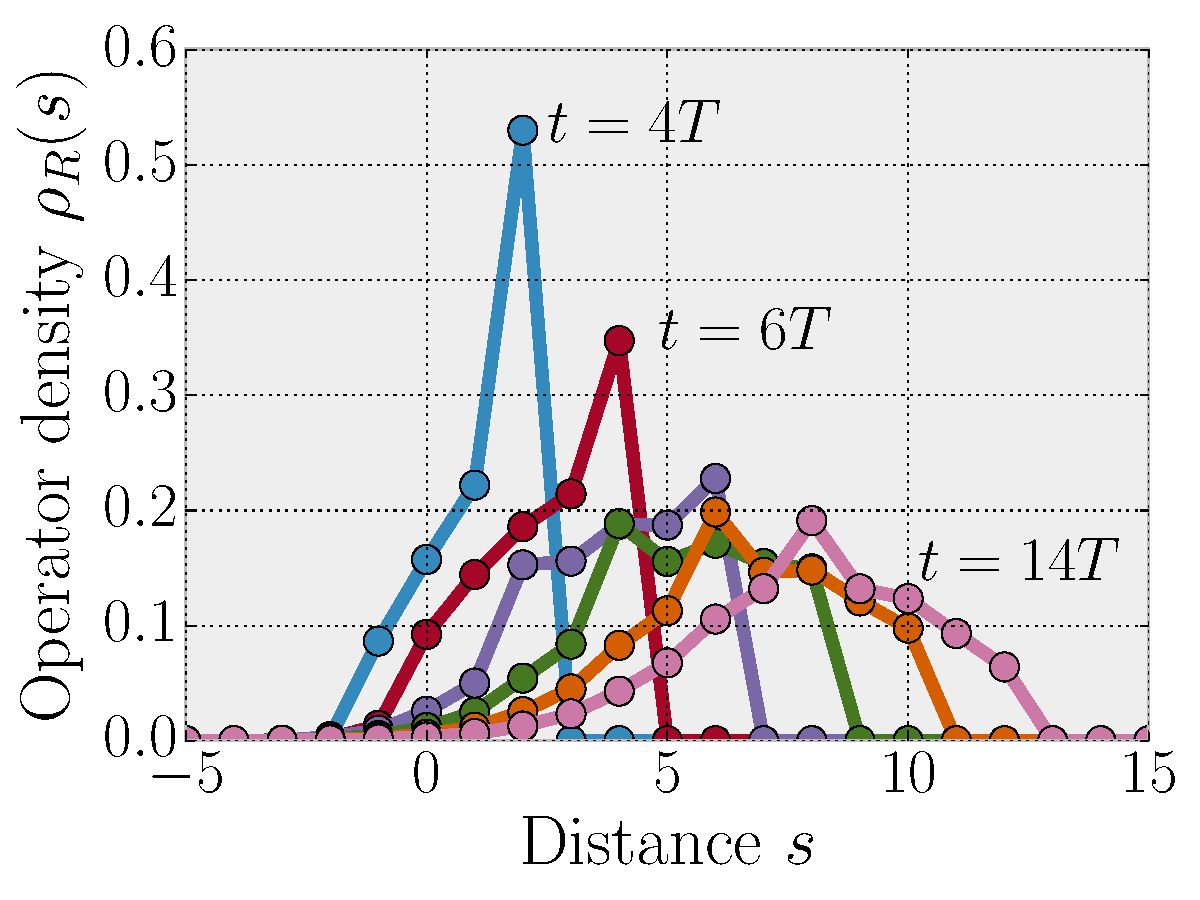
\includegraphics[width=.3\textwidth]{vonKpeaks}
	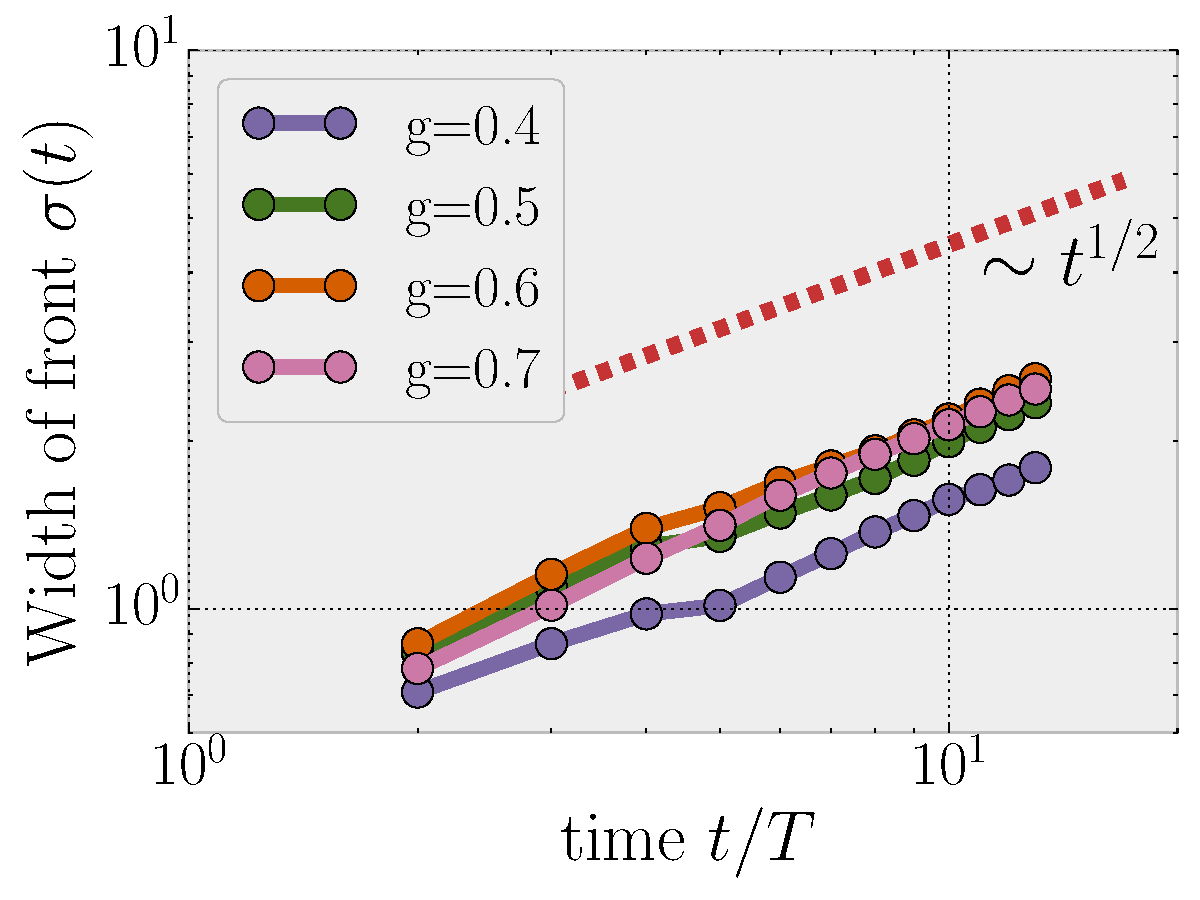
\includegraphics[width=.3\textwidth]{vonKalpha}
	\caption{Spreading of peaks in the kicked Ising model~\cite{vonKeyserlingkHydro}.}
	\label{fig:vonKalpha}
\end{figure}
Fig.~\ref{fig:vonKalpha} shows that $\alpha\approx .5$, so that the peaks spread with $\sqrt{t}$. This will be another test of our quantum circuits.

\subsection{Circuits with no conservation laws} \label{sub:cncons}

Early exponential growth.
Presence of front.
Broadening of front and exponential dependence therein.

The circuit under investigation in this section has the same architecture as Fig.~\ref{fig:circuit}, with each gate chosen from the Haar measure. Our goal is to find the dynamics of $\rho_R$ under the action of the full circuit, and our analysis will follow~\cite{vonKeyserlingkHydro}. The first step in doing so is to calculate the dynamics of $\rho_R$ under a single gate. 

We want to calculate $\rho_R(i,\tau+1)$ and $\rho_R(i+1, \tau+1)$ (Fig.~\ref{fig:2sites}). It should be clear that these quantities only depend on $\rho_R(i,\tau)$ and $\rho_R(i+1, \tau)$. In fact it is even simpler, in that $\rho_R(i,\tau+1)$ and $\rho_R(i+1, \tau+1)$ only depend on the sum $\rho_R(i,\tau) + \rho_R(i+1, \tau)$. 

\begin{figure}
	\centering
	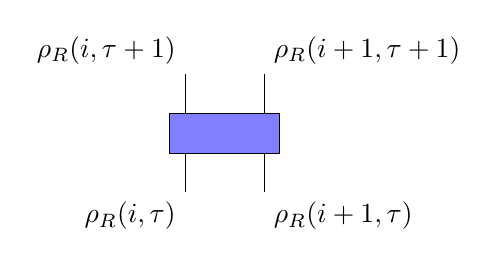
\begin{tikzpicture}[scale = 1]
\draw (0,0) node[below left]{$\rho_R(i,\tau)$} -- (0,1.5) 
			node[above left]{$\rho_R(i,\tau+1)$};
\draw (1,0) node[below right]{$\rho_R(i+1,\tau)$} -- (1,1.5)
			node[above right]{$\rho_R(i+1,\tau+1)$};

\filldraw[color=black, fill=blue!50] (-.2,.5) rectangle (1.2,1);


\end{tikzpicture}
	\caption{Diagram of the operator weights before and after the application of the gate. Values at $\t+1$ are calculated in the text.}
	\label{fig:2sites}
\end{figure}

Looking at $\rho_R(i,\tau)$ and $\rho_R(i+1, \tau)$ is equivalent to looking only at Pauli strings which are $I$ on all sites past $i+1$ but are non-identity on either $i$ or $i+1$ (or both).
This leaves us with $q^4-1$ two-site operators to consider. The Haar-random gate transforms any of these operators to any other with equal probability~\cite{BrownScrambling}, regardless of whether the initial operator was an identity on site $i+1$. This is why the final values only depend on $\rho_R(i,\tau) + \rho_R(i+1, \tau)$.

Of the $q^4+1$ final operators, $q^2-1$ are the identity on site $i+1$. These operators contribute to $\rho_R(i,\tau+1)$, while the rest contribute to $\rho_R(i+1, \tau+1)$. In other words the weight moves to site $i$ with probability $p_\text{back} = \frac{q^2-1}{q^4-1} = \th{q^2+1}$ or moves forward with probability $p\equiv 1- p_\text{back} = \frac{q^2}{q^2+1}$. Thus
\begin{align}
\rho(i,\t+1) &= (1-p)\left[\rho(i,\t)+\rho(i+1,\t)\right],\nn
\rho(i+1,\t+1) &= p\left[\rho(i,\t)+\rho(i+1,\t)\right].
\end{align}
This is true at each individual gate. If there were a gate at each site at each time, this would be the final word. However, since the dynamics will only be periodic in every two layers of the circuit, we must calculate the dynamics for two layers to get the whole picture.

To do so, we will define some dense but useful notation. Since the sum of weights at consecutive sites is so important, we will abbreviate it as
\begin{align}
\tilde{\rho}_R(i,\t) \equiv \rho_R(i,\tau) + \rho_R(i+1, \tau). \label{eqn:rhotil}
\end{align}
Now, referring to Fig.~\ref{fig:4sites}, 
\begin{figure}
	\centering
	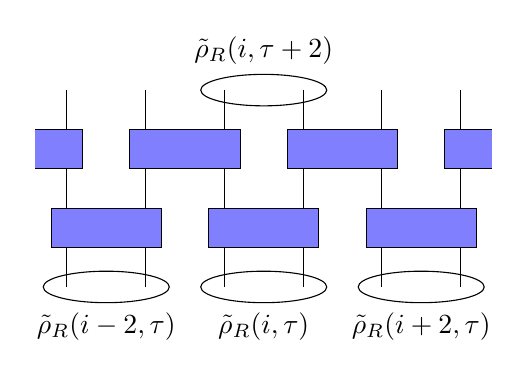
\begin{tikzpicture}[scale = 1]
\draw (0,0) -- (0,2.5);
\draw (1,0) -- (1,2.5);
\draw (2,0) -- (2,2.5);
\draw (3,0) -- (3,2.5);
\draw (4,0) -- (4,2.5);
\draw (5,0) -- (5,2.5);

\foreach \x/\y in {0/1, 2/1, 4/1, 1/2, 3/2} 
\filldraw[color=black, fill=blue!50] (\x-.2,\y-.5) rectangle (\x+1.2,\y);

\draw (0.5,0) circle [x radius=.8, y radius=.2];
\draw (0.5,-0.2) node[below]{$\tilde{\rho}_R(i-2,\t)$};
\draw (2.5,0) circle [x radius=.8, y radius=.2];
\draw (2.5,-0.2) node[below]{$\tilde{\rho}_R(i,\t)$};
\draw (2.5,2.5) circle [x radius=.8, y radius=.2];
\draw (2.5,2.7) node[above]{$\tilde{\rho}_R(i,\t+2)$};
\draw (4.5,0) circle [x radius=.8, y radius=.2];
\draw (4.5,-0.2) node[below]{$\tilde{\rho}_R(i+2,\t)$};

\draw[fill=blue!50] (-.4,1.5) -- (.2,1.5) -- (.2,2) -- (-.4,2);
\draw[fill=blue!50] (5.4,2) -- (4.8,2) -- (4.8,1.5) -- (5.4,1.5);

\end{tikzpicture}
	\caption{Operator weights after two layers of the circuit}
	\label{fig:4sites}
\end{figure}
we have

These results can be summarized in Fig.~\ref{fig:vonKSpreading}.
\begin{figure}
	\centering
	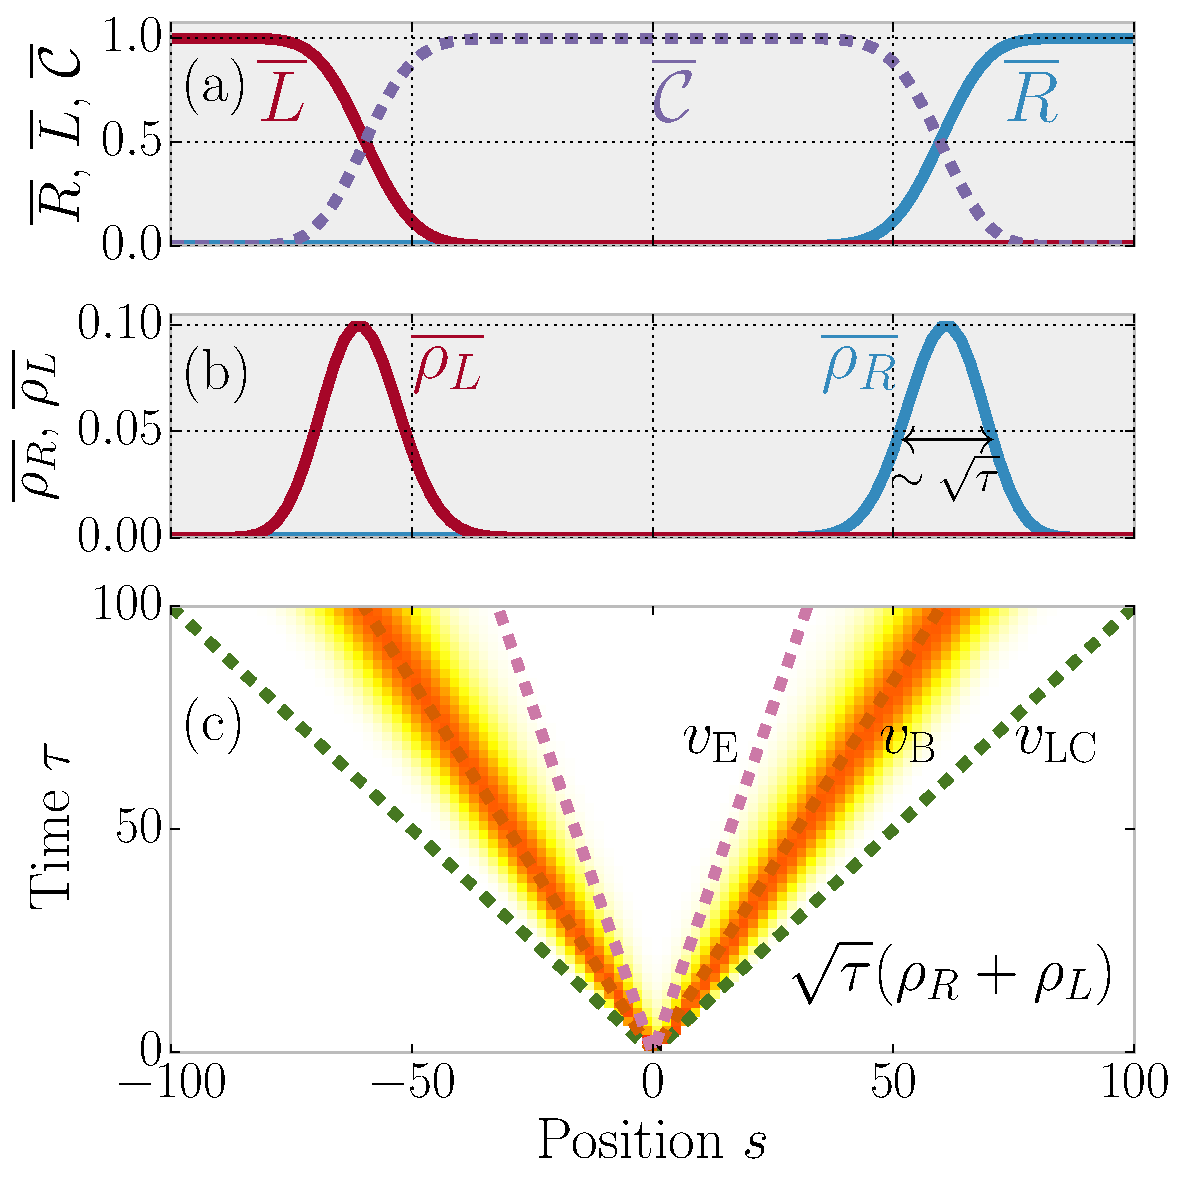
\includegraphics[width=.5\textwidth]{vonKSpreading}
	\caption{Spreading of an initially local operator under a quantum circuit with no conservation laws~\cite{vonKeyserlingkHydro}.}
	\label{fig:vonKSpreading}
\end{figure}


\section{Thermalization in systems with conservation laws} \label{sec:cons}

Introducing conserved charges to our systems slows down their dynamics. In this section we will see how this process occurs, in both physical systems and quantum circuits. It is straightforward to introduce conserved charges to the circuits by restricting to gates that satisfy some conservation law. For the physical systems we have two ways to proceed. We can either consider Floquet systems with conservation laws, or systems with time-independent Hamiltonians (with or without further conservation laws).

\subsection{Floquet systems with conserved quntities} \label{sub:fcons}

We can introduce conserved charges to Floquet systems by ensuring that both partial Hamiltonians in the model obey some conservation law. Ref.~\cite{KhemaniOpSp} studies a model with time evolution operator
\begin{align}
U_F(T)=e^{i\frac{T}{2}H_z}e^{i\frac{T}{2}H_{xy}},
\end{align}
where
\begin{align}
H_z &= J_z\sum_i Z_iZ_{i+1},\nn
H_{xy} &= J_{xy}\sum_i\left[X_iX_{i+1}+Y_iY_{i+1}\right].
\end{align}

\note{In these ``physical systems," it is possible to have approximately conserved charges, i.e. on the localized side of a phase transition\dots}


\section{Fractonic systems} \label{sec:frac}

In this section we will explore various fractonic systems. We will start with exactly solvable models and show that these naturally result in massive (gapped) fractons. However we will quickly transition to tensor gauge theory, where we can create gapless fractons. Ultimately, we want to show the connection between multipole conservation laws (specifically dipole) and fractons. This motivates the study of random circuits that conserve dipole moment as a setting for localized charges, which will be presented in Sec.~\ref{sec:fraccirc}.

\subsection{Tensor gauge theory} \label{sub:tensor}

Make sure to use~\cite{PretkoFractonGauge}.

Another way to create fractons is through symmetric tensor gauge theory. This method will be the most useful for our purposes. We will start with a lightning review of electromagnetism simply for the sake of notation, and show why considering tensors results in conservation of higher moments of charge. 

Nonrelativistically, electromagnetism can be described with the Lagrangian \cite{TongQft}
\begin{align}
\mathcal{L} = -\th{4}F_{\mu\nu}F^{\mu\nu} + j^\mu A_\mu.
\end{align}
We can derive conservation of charge from the equations of motion\dots (Something happens here where we have to use the gauge freedom instead but I haven't totally worked this out yet.)

Consider generalizing from a vector potential $A_{i}$ to a tensor potential $A_{ij}$ which can be decomposed into a trace and symmetric and antisymmetric parts, $A_{ij} = k\delta_{ij} + \tilde{\omega}_{ij} + A'_{ij}$. The first term\dots. The second term can be rewritten as a vector potential, so it will have the same dynamics as electromagnetism. That leaves with only the symmetric tensor, which we will relabel $A_{ij}$.

(Somehow\dots) the gauge transformation $A_{ij}\to A_{ij}+\partial_i\partial_j\alpha$ gives the constraint 
\begin{align}
\partial_i\partial_jE_{ij}=\rho.\label{eqn:dipole}
\end{align}
Once again, we have conservation of charge:
\begin{align}
\int_V\rho dV = \int_V \partial_i\partial_j E_{ij}dV = \int_{\partial V}n_i\partial_jE_{ij}dA,
\end{align}
which says that charge cannot be produced locally. It must instead come in through the boundary. We also have a new conservation law
\begin{align}
\int_Vx_i\rho dV = \int_V x_i\partial_j\partial_k E_{jk}dV = \text{boundary terms},
\end{align}
where the boundary terms come from both partial integration and Stokes' theorem~\cite{NandkishoreFractons}.

(I don't have a good understanding of this process yet but I'll refer to~\cite{PretkoSubdim, RasmussenYouXu, SlagleTensor}.)

The conservation of dipole moment means that an isolated charge cannot move without creating an isolated dipole somewhere else, which costs energy. Thus, the charges are immobile in the low-energy limit. 

(I'll then discuss this model more, including the difference between the discrete and continuous cases. I'll also present some of the connections to elasticity and gravity, such as in~\cite{PretkoElasticity}.)


\section{Localization in fractonic circuits} \label{sec:fraccirc}

This section will mostly cover the results in~\cite{PaiFracton}. I'll go through their analytic results and show that their numerics match up. I'd prefer not to do my own numerics because I assume anything I can do in the next month and a half will be a subset of what they achieved, but if you think my essay would benefit from some validation of their numerics at lower $L$, then I'll go for it. 


\section{Results and Conclusions} \label{sec:conc}

%%%%%%%%%%%%%%%%%%%%%%%%%%%%%%%%%%%%%%%%%%%%%%%%%%%%%%%%%%%%%%%%%%
%\printbibliography
%%%%%%%%%%%%%%%%%%%%%%%%%%%%%%%%%%%%%%%%%%%%%%%%%%%%%%%%%%%%%%%%%%
\nocite{apsrev41Control}
\bibliography{../global,revtex-custom}
%%%%%%%%%%%%%%%%%%%%%%%%%%%%%%%%%%%%%%%%%%%%%%%%%%%%%%%%%%%%%%%%%%

\end{document}
